\subsection{Trigger for the electron final states}
\label{subsec:trigger-for-electron}

The trigger used for the selection of the electron final state are mainly
described in Sec.~4.2.5 in~\ref{ATL-DAQ-PUB-2019-001}.

[Text and plots from ATL-DAQ-PUB-2019-001 to have a starting point]\\
In 2018, a new set of triggers was added to select low-\pT dielectron events within an
invariant mass region corresponding to decays of $b$-hadrons. The development focused on
$B^{0}\rightarrow K^{*} e^{+}e^{-}$ decays, but all triggers developed are agnostic to
additional tracks, and thus are also sensitive to \emph{e.g.}
$B^{+}\rightarrow K^{+} e^{+}e^{-}$ decays.

Both L1 items and HLT algorithms were developed.
% L1_BPH-0M9-EM7-EM5
% L1_BPH-0DR3-EM7J15
Mimicking the $B$-physics L1 muon strategy, L1 topological triggers using EM RoIs were developed.
The main trigger requires the invariant mass between two L1 EM RoIs, one with $\ET > 7$~GeV (EM7)
and the second with $\ET > 5$~GeV (EM5), to be less than 9~GeV.
However, since the granularity of the L1 calorimeter trigger is somewhat coarser than the extent
of a single, low-\pT electron, when the two electrons are very close-by they will only create
a single L1 EM RoI in the detector.  Thus, a L1 trigger for close-by electrons was created,
which requires a L1 EM RoI within $\Delta R < 0.3$ of a L1 jet RoI.
These two situations are depicted in Figure~\ref{fig:BeeK_sketch}.

\begin{figure}[htbp]
  \centering %trim = 0.9cm 0 1.5cm 0, clip,
  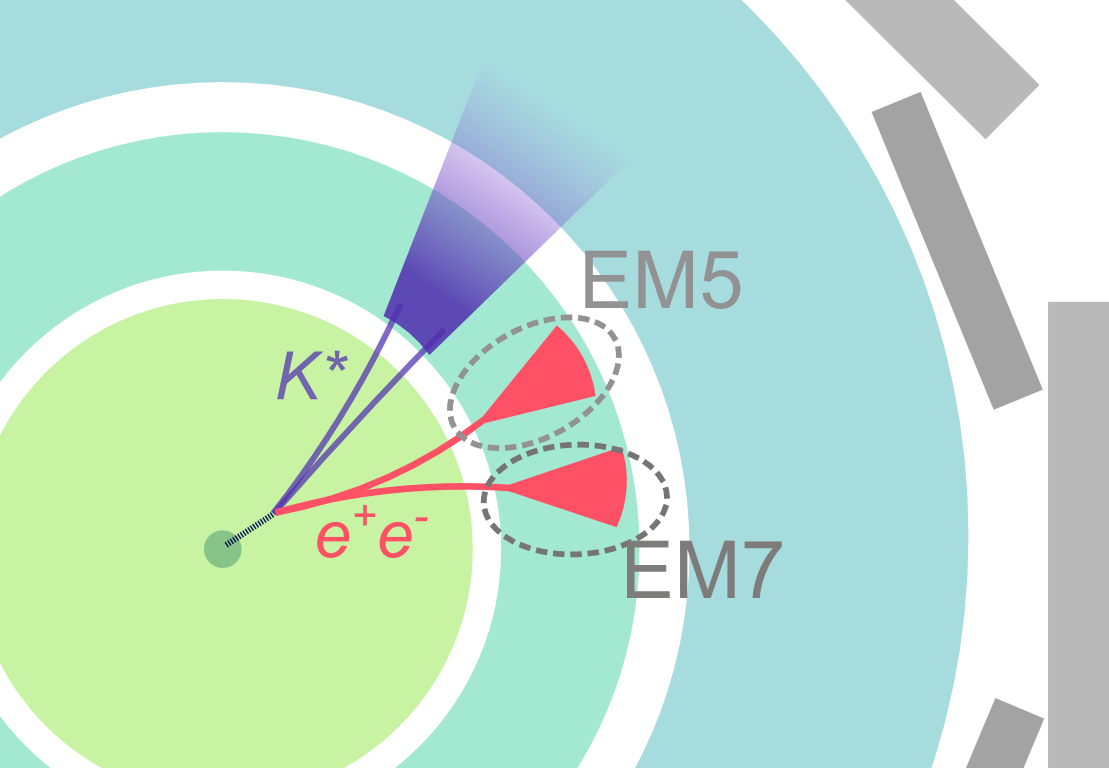
\includegraphics[width=.35\textwidth]{figures/BtoKstaree_separated}
  ~~~~~~~~~~~~
  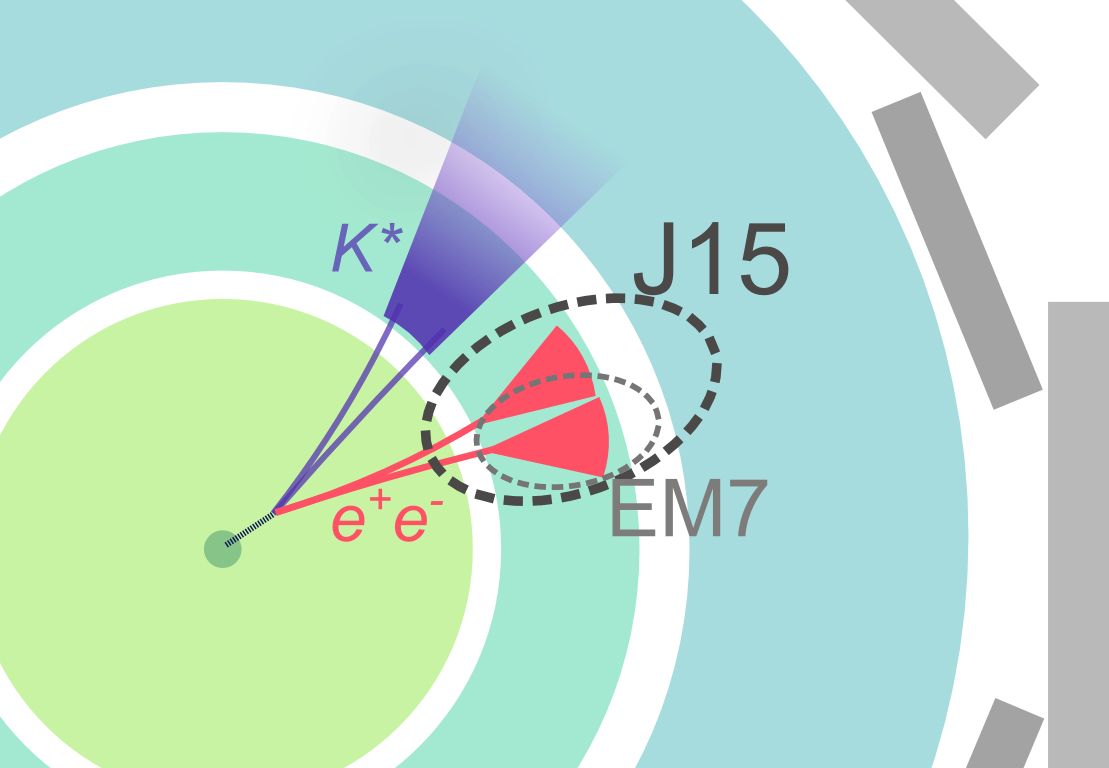
\includegraphics[width=.35\textwidth]{figures/BtoKstaree_close}
  \caption{
    Topological sketches of $B\rightarrow K^{*} e^{+}e^{-}$ decays, where, from the point of view of
    the L1 EM RoIs, the two electrons are well-separated (left), and the two electrons are overlapping
    (right). From the centre outwards, the colours represent the inner detector, electromagnetic
    calorimeter, hadronic calorimeter, and first layer of the muon spectrometer.
  }
  \label{fig:BeeK_sketch}
\end{figure}

On their own, the rates of these two L1 triggers are greater than the global 100 kHz limit,
and thus they are combined with a muon requirement to lower the rate: either one MU6 muon or
two MU4 muons. Because the production of one $b$-hadron is likely to result in the production
of another, the muon requirement provides a higher purity sample than simply prescaling
the original L1 triggers. The rates of the two L1 EM-based triggers with and without
combination with the L1 muon selections are shown in Figure~\ref{fig:BeeK_L1Rates}.

\begin{figure}[htbp]
  \centering %trim = 0.9cm 0 1.5cm 0, clip,
    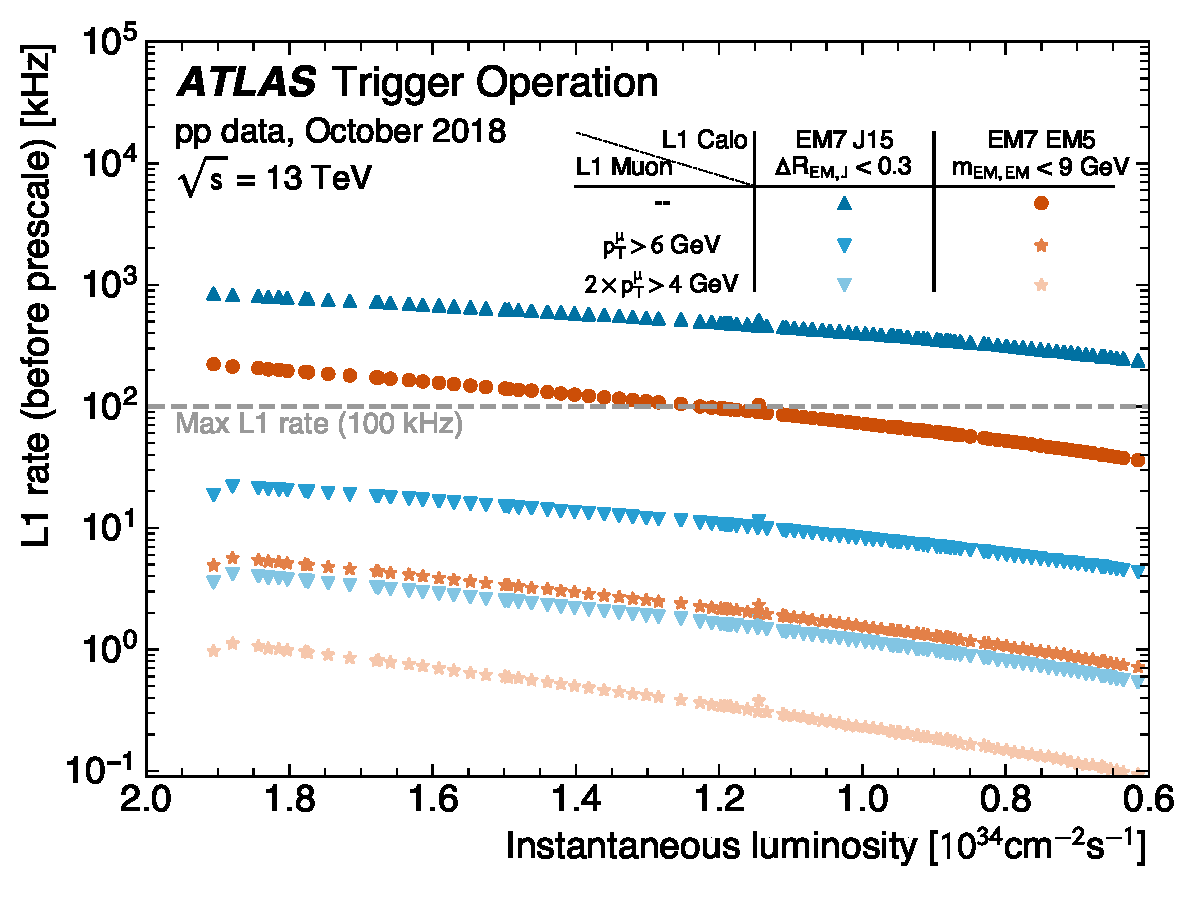
\includegraphics[width=.65\textwidth]{figures/L1BPH_rates_ATLASStyle}
  \caption{
  L1 trigger rate, before the application of any prescale, as a function of instantaneous
  luminosity for the two L1 items targeting $B\rightarrow K^{*} e^{+}e^{-}$ decays alone
  and in association with either one 6~GeV muon or two 4~GeV muons. The L1 calorimeter-based
  thresholds for an EM RoI with $\ET > 5$~GeV, an EM RoI with $\ET > 7$~GeV, and a jet RoI
  with $\ET > 15$~GeV, are represented by EM5, EM7, and J15, respectively.
  The four triggers with an L1 muon requirement were deployed online, with end-of-fill prescale strategies.
  }
  \label{fig:BeeK_L1Rates}
\end{figure}

For the L1 trigger with two L1 EM RoIs, two electrons matching the L1 EM RoIs are required
in the HLT, with $\ET^{1} >  9$~GeV and $\ET^{2} > 5$~GeV. For the single L1 EM RoI trigger,
two HLT electrons with 5~GeV are required. The HLT electrons were required to pass a very
loose electron likelihood (LH) PID~\cite{ATLAS-CONF-2016-024}, without any requirement on
the transverse impact parameter. The electrons are required to form a vertex with $\chi^2 < 20$,
and the invariant mass of the vertex must be between 0.1 and 6~GeV, which is inclusive
of all relevant $b$-hadron decays. Additionally, HLT muons are required in parallel with
the L1 muon requirement (either one 6~GeV or 2, 4~GeV HLT muons). These four triggers were
deployed on 8 June 2018. An end-of-fill strategy was applied to all triggers except the
one with 2, 4~GeV muons and electron thresholds of 9~GeV and 5~GeV, to account for the large L1 rates.

Due to the additional muon requirement, the aforementioned triggers were not fully efficient
for signal events, and thus a second set of triggers was developed without the muon requirement.
However, as demonstrated in Figure~\ref{fig:BeeK_L1Rates}, running electron-only items
at L1 was not feasible. Thus, instead of requiring dedicated L1 triggers, an HLT trigger
was instead run over every event selected by the L1 trigger (L1 accept). HLT electron
reconstruction was seeded from EM3 RoIs and two separate triggers were used, one for
well-separated electrons and one for close-by electrons. In both cases, two 5~GeV HLT electrons
passing a very loose electron LH PID, without any requirement on the transverse impact parameter,
are required, with the same vertex requirements as the seeded triggers. It should be noted that,
although this trigger ran without an HLT prescale, it only ran if there was an L1 accept
from the rest of the trigger menu. %However, the L1 accept is biased towards high-\pT physics\
 and thus provides a hard scatter-enriched environment that is more likely to contain
 signal events than any given event with low-\pT EM~RoIs. [speculation]

\begin{figure}[h!]
  \centering %trim = 0.9cm 0 1.5cm 0, clip,
  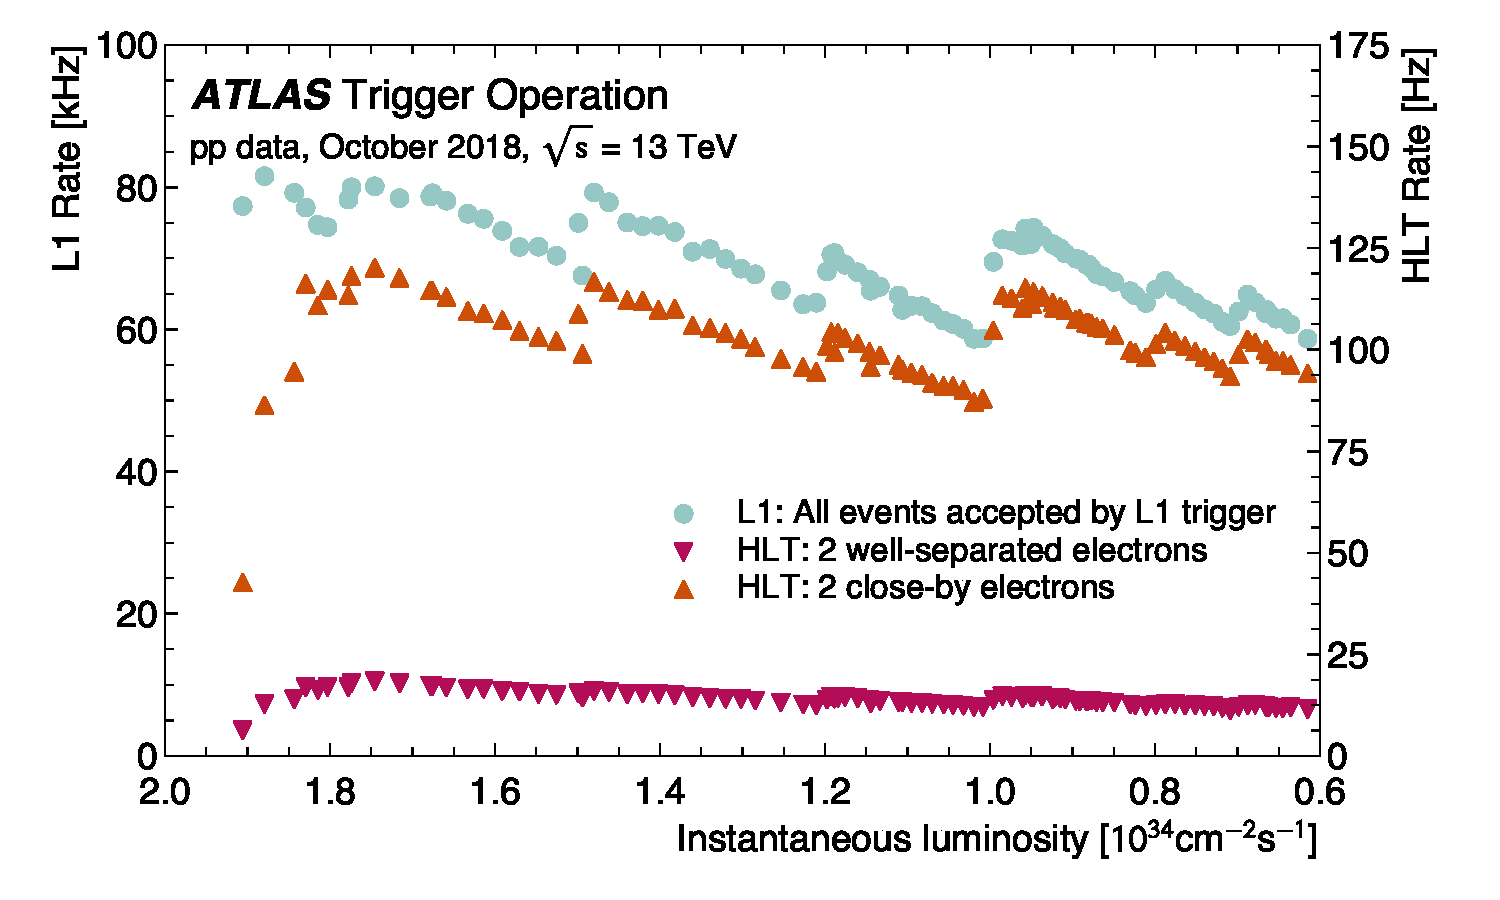
\includegraphics[width=0.65\textwidth]{figures/BeeK_OctOnly_ATLAS}
  \caption{L1 and HLT trigger rates as a function of instantaneous luminosity for the two
  unseeded triggers targeting $B\rightarrow K^{*} e^{+}e^{-}$ decays.
  }
  \label{fig:BeeK_HLT_unseeded}
\end{figure}

These unseeded triggers were deployed on 14~July~2018, and ran without any HLT prescale below
luminosities of \lumi{1.85}. Above this, small HLT prescales were applied to reduce the
excessive pressure on the readout system required to run low-\pT electron reconstruction
in every event accepted by the L1 trigger: 5 above \lumi{2}, 2.5 between \lumi{1.95} and
\lumi{2}, and 1.5 between \lumi{1.85} and \lumi{1.95}. These HLT prescales were achieved
by online adjustments until the optimal running scenario was achieved.
Figure~\ref{fig:BeeK_HLT_unseeded} shows the L1 accept rate and HLT rates of each of the
two unseeded triggers as a function of instantaneous luminosity, for a run in October 2018.
